\documentclass[letterpaper,12pt]{article}
\usepackage{tabularx} % extra features for tabular environment
\usepackage{amsmath}  % improve math presentation
\usepackage{float}
\usepackage{pdfpages}
\usepackage{graphicx} % takes care of graphic including machinery
\graphicspath{ {./figures/} }
\usepackage[margin=1in,letterpaper]{geometry} % decreases margins
 % takes care of citations
\usepackage[final]{hyperref} % adds hyper links inside the generated pdf file
\hypersetup{
	colorlinks=true,       % false: boxed links; true: colored links
	linkcolor=blue,        % color of internal links
	citecolor=blue,        % color of links to bibliography
	filecolor=magenta,     % color of file links
	urlcolor =blue         
}




\begin{document}

\title{EXPERIMENT\protect\\"LIGHT DEPENDENT RESISTORS AND DISTANCE MEASUREMENTS"}
\author{Prepared by Ahmet Akman 2442366}
\date{\today}
\maketitle
\section*{Objectives}
\begin{itemize}
	\item The Light Dependent Resistor (LDR) component to be characterized.
	\item Distance measurement sensor mechanisms to be indtroduced.
\end{itemize}
\section*{Preliminary Work}
\subsection*{1}
Watch the  videos (provided in Appendix).
\subsection*{2}
Study "Notes on Multimeters".
\subsection*{3}
Light Dependent Resistors (abrevieted as LDRs) are semiconductor based electronic component. An example of an LDR is shown in Figure 1. 
\begin{figure}[H]
	\centering
	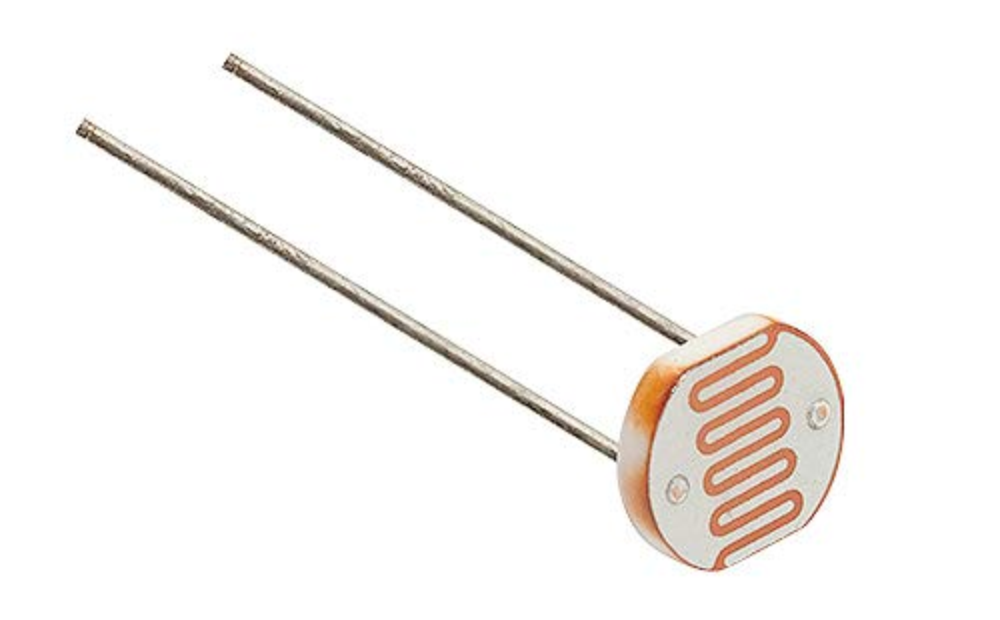
\includegraphics[width=0.5\textwidth]{LDR_photo.png}
	\caption{LDR picture}
\end{figure} 
LDR ,as easily can be inferred from its name, has a variable resistance which depends on the illumination on its surface. So, its resistance is high in dark and low in light. Those resistance values are vastly dependent on the size and the model of the particular LDR. In this step you are required to find an LDR from a manufacturer and from the datasheet provide following informations with necessary plots. You do not need to explain those data, it is enough to provide in the preliminary report with appropriate format.
\begin{itemize}
	\item Sensitive surface area.
	\item Resistance as a function of illumination (with plot).
	\item Spectral response (with plot). 
\end{itemize}   
\subsection*{4}
The schematic symbol of LDR component is given in Figure 2.
\begin{figure}[H]
	\centering
	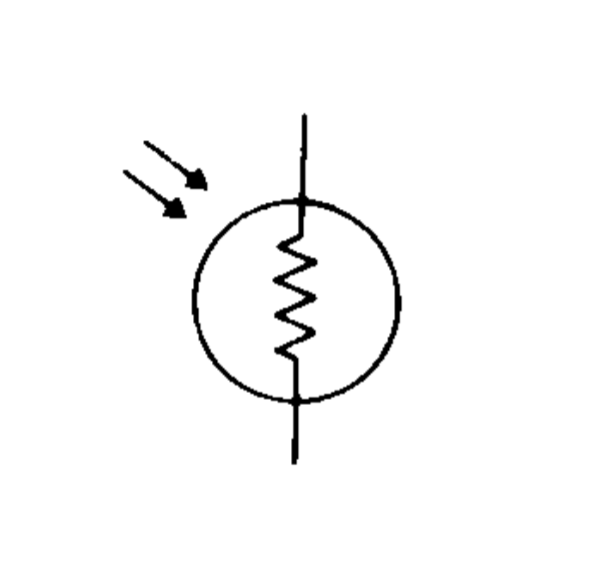
\includegraphics[width=0.5\textwidth]{LDR_symbol.png}
	\caption{LDR schematic symbol}
\end{figure} 
Using this information, briefly describe the functional behavior of the circuit given in Figure 3. (\textbf{Hint:} It would be nice to look back to comparator op-amp setup.)
\begin{figure}[H]
	\centering
	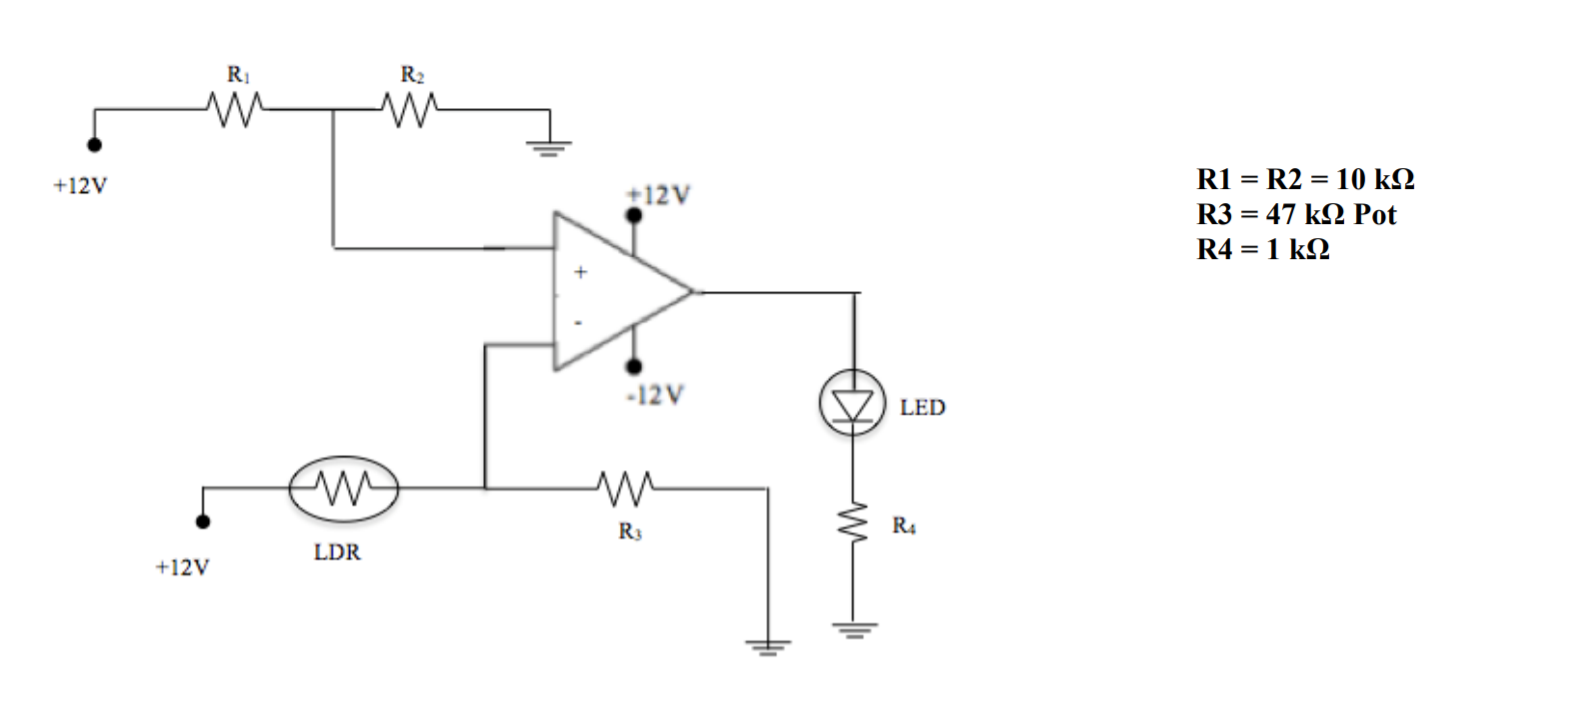
\includegraphics[width=1\textwidth]{darkness.png}
	\caption{A circuit with LDR}
\end{figure} 

\subsection*{5}
For this step you are required to do small research about optical distance sensors. Independent from the experiment, this step is for you to gain an insight on optical distance sensors.
\begin{itemize}
	\item Describe how triangulation measurement method works in \(\sim\) 50-100 words with a credible source. 
	\item Describe how time of flight (ToF) measurement method works in \(\sim\) 50-100 words with a credible source. 
	\item Describe how phase measurement method works in \(\sim\) 50-100 words with a credible source. 
\end{itemize}
\section*{Equipment List}
\begin{itemize}
	\item LDR (Light Dependent Resistor)
	\item Digital Multimeter.
	\item Ruler.
	\item A bright light source like a phone flashlight. (This is expected to be supplied from the student.)
\end{itemize}
\section*{Experimental Work}
Important note - 1: You only need to show your work to the lab assistant for step 2.
\subsection*{Step 1}
Describe the relation between illumination on a surface and the distance of the light source.
\subsection*{Step 2}
In this step you are required to measure the distance of a light source using LDR component. Setup the configuration given in Figure 4 by connecting the probes to the digital multimeter. Adjust the multimeter so that it measures the resistance. 
\begin{figure}[H]
	\centering
	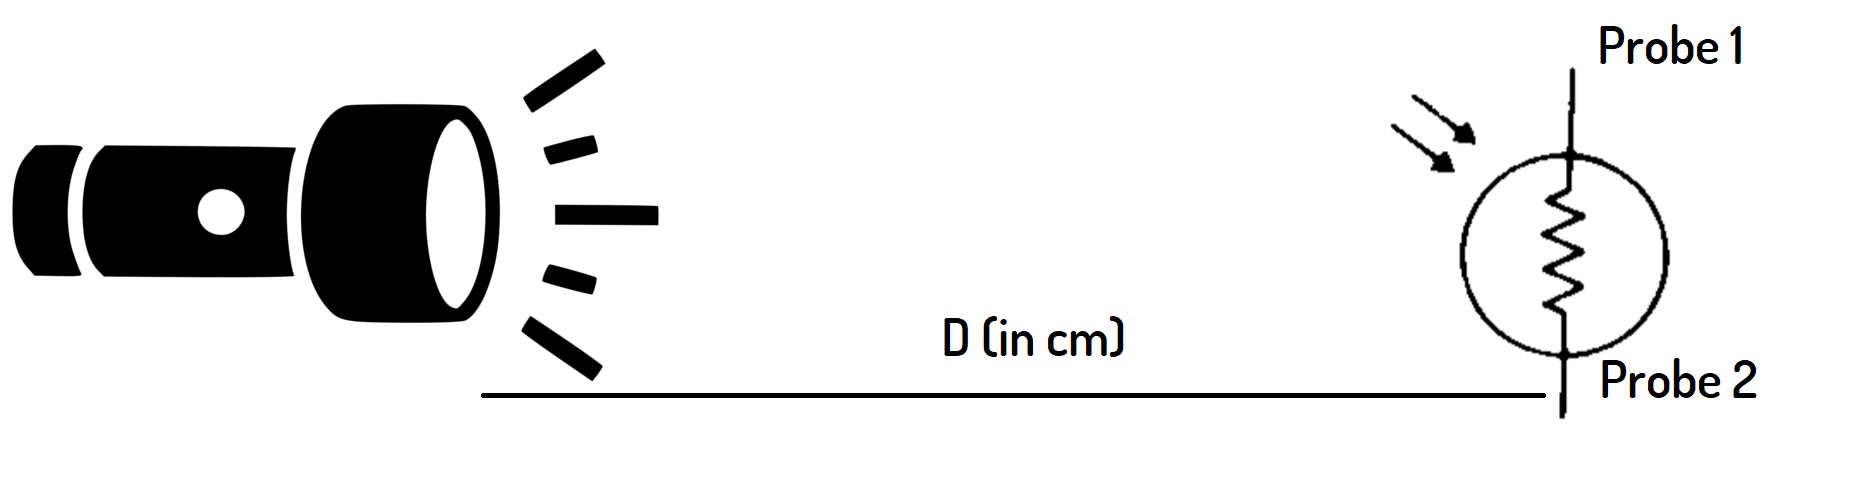
\includegraphics[width=1\textwidth]{setup.png}
	\caption{Simple distance measurement with LDR configuration}
\end{figure}
It is necessary to align the source with  the surface of the LDR for better measurements. Also, pay attention not to  cause the ambient light to fluctuate with shadows.
\subsubsection*{a}
Using ruler make the distance D as "15 centimeter". Then record the resistance value. Using this value solve the following equation. Determine the  constant.

%\begin{abstract}
%abstract
%\end{abstract}

\section{Introduction and Project Objective}
This document presents the design approaches proposed for the given term project of EE213. The term-project requirements can be basically summarized that students are expected to design an experiment to measure the distance of a light source. It is given that the component "LDR (Light Dependent Resistor)" will be used as the sensor element. Also, the basic passive components, Op-Amps, and laboratory equipment are in the scope of use. The physical appearance of a photoresistor is given in Figure 1. 
\section{Conclusion}
In conclusion, two proposed measurement methods are discussed in terms of preliminary measurements and inferences. Both methods have pros and cons. The first method is easier to build, but its accuracy is a matter of question since it is directly related to the resistance value. The second method seems more complicated, but it promises accuracy and includes proper laboratory work. On the contrary, the requirement for the precise time intervals method has the possibility to fail in laboratory conditions. There are strong light source dependencies for both methods, but the second method includes the elimination of this dependency in a sense. Further investigations will be done, and one of the methods will be chosen for the laboratory manual. To sum up, there are proposed two different approaches for the measurement of the distance of a light source, and they are evaluated.   





\end{document}


\begin{table}[H]
	\begin{center}
		\caption{Resistance reading by color code convention.}
		\vspace{2mm}
		\begin{tabular}{||c | c | c||} 
		 \hline
		 Color Order & Value & Tolerance \\ [0.5ex] 
		 \hline\hline
		 Brown / Black / Red / Gold & 1k\( \Omega \) & \( \% \) 5  \\ 
		 \hline
		 Yellow / Violet / Red / Gold & 4.7k\( \Omega \) & \( \% \) 5   \\
		 \hline
		 Brown / Grey / Orange / Gold & 18k\( \Omega \) & \( \% \) 5  \\ [1ex] 
		 \hline
		\end{tabular}
	\end{center}
	\end{table}

\begin{figure}[H]
	\centering
	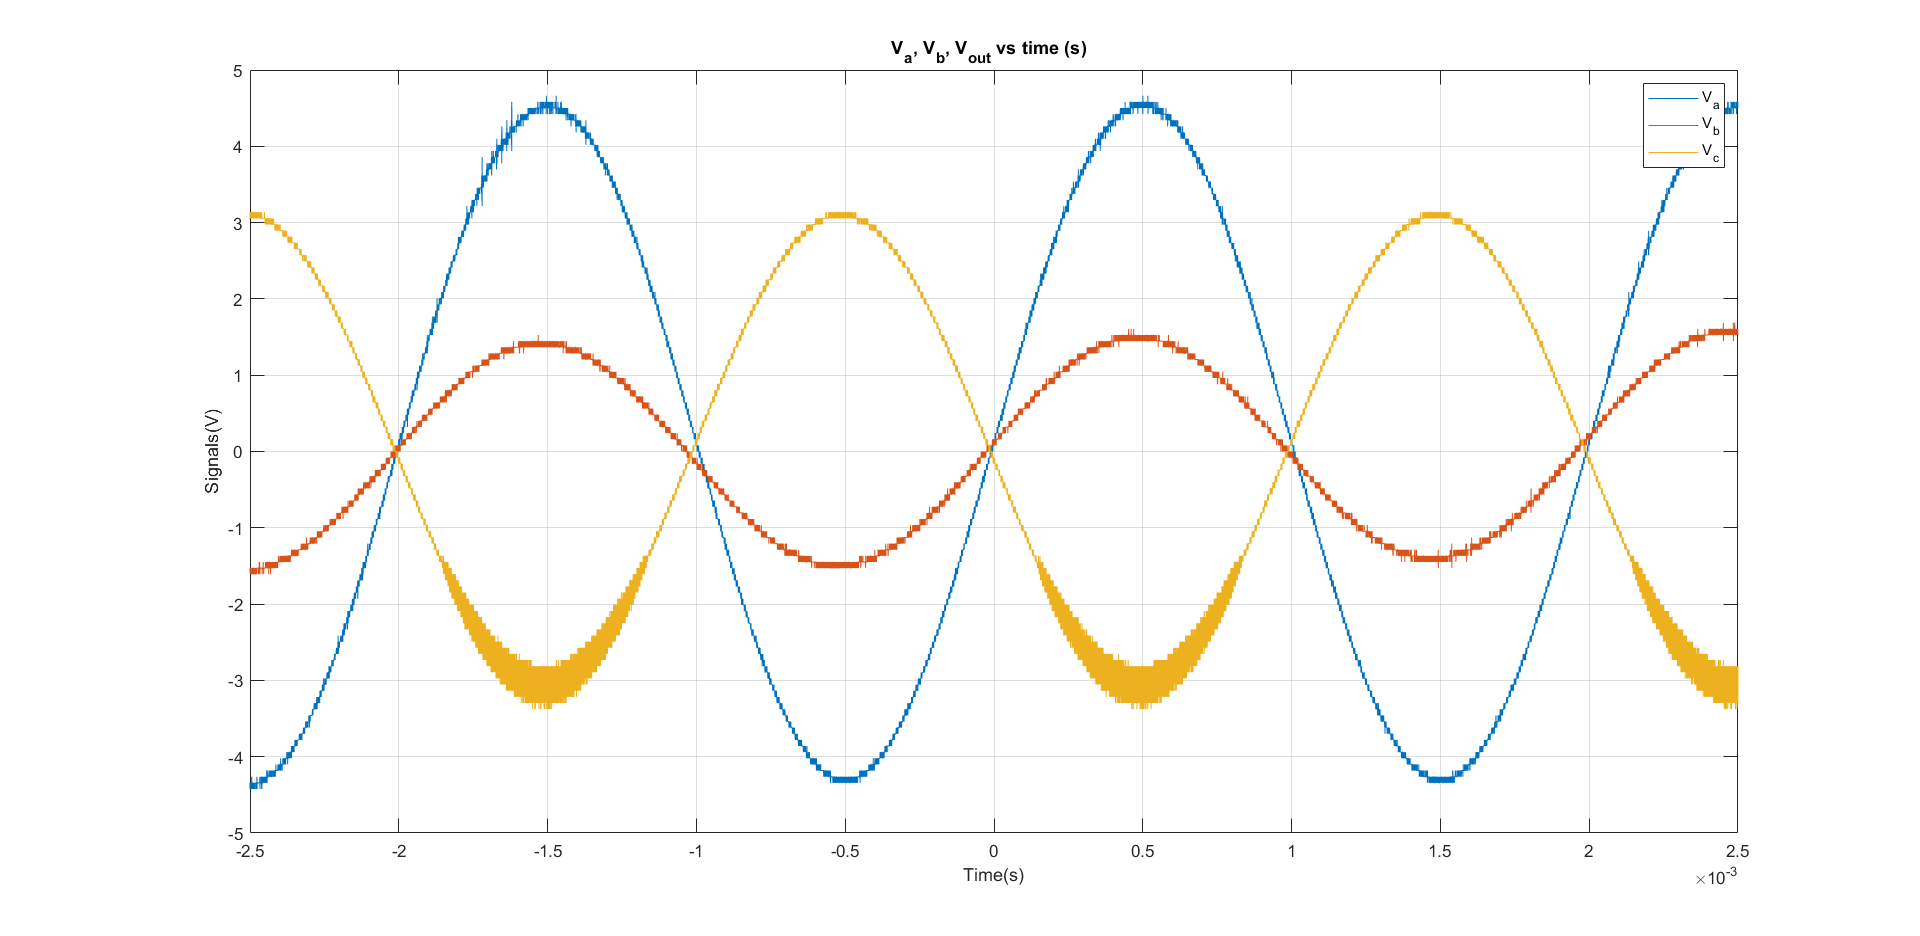
\includegraphics[width=0.6\textwidth]{5.png}
	\caption{Circuit schematic for the step 5}
\end{figure} 

	\begin{figure}[htp] \centering{
		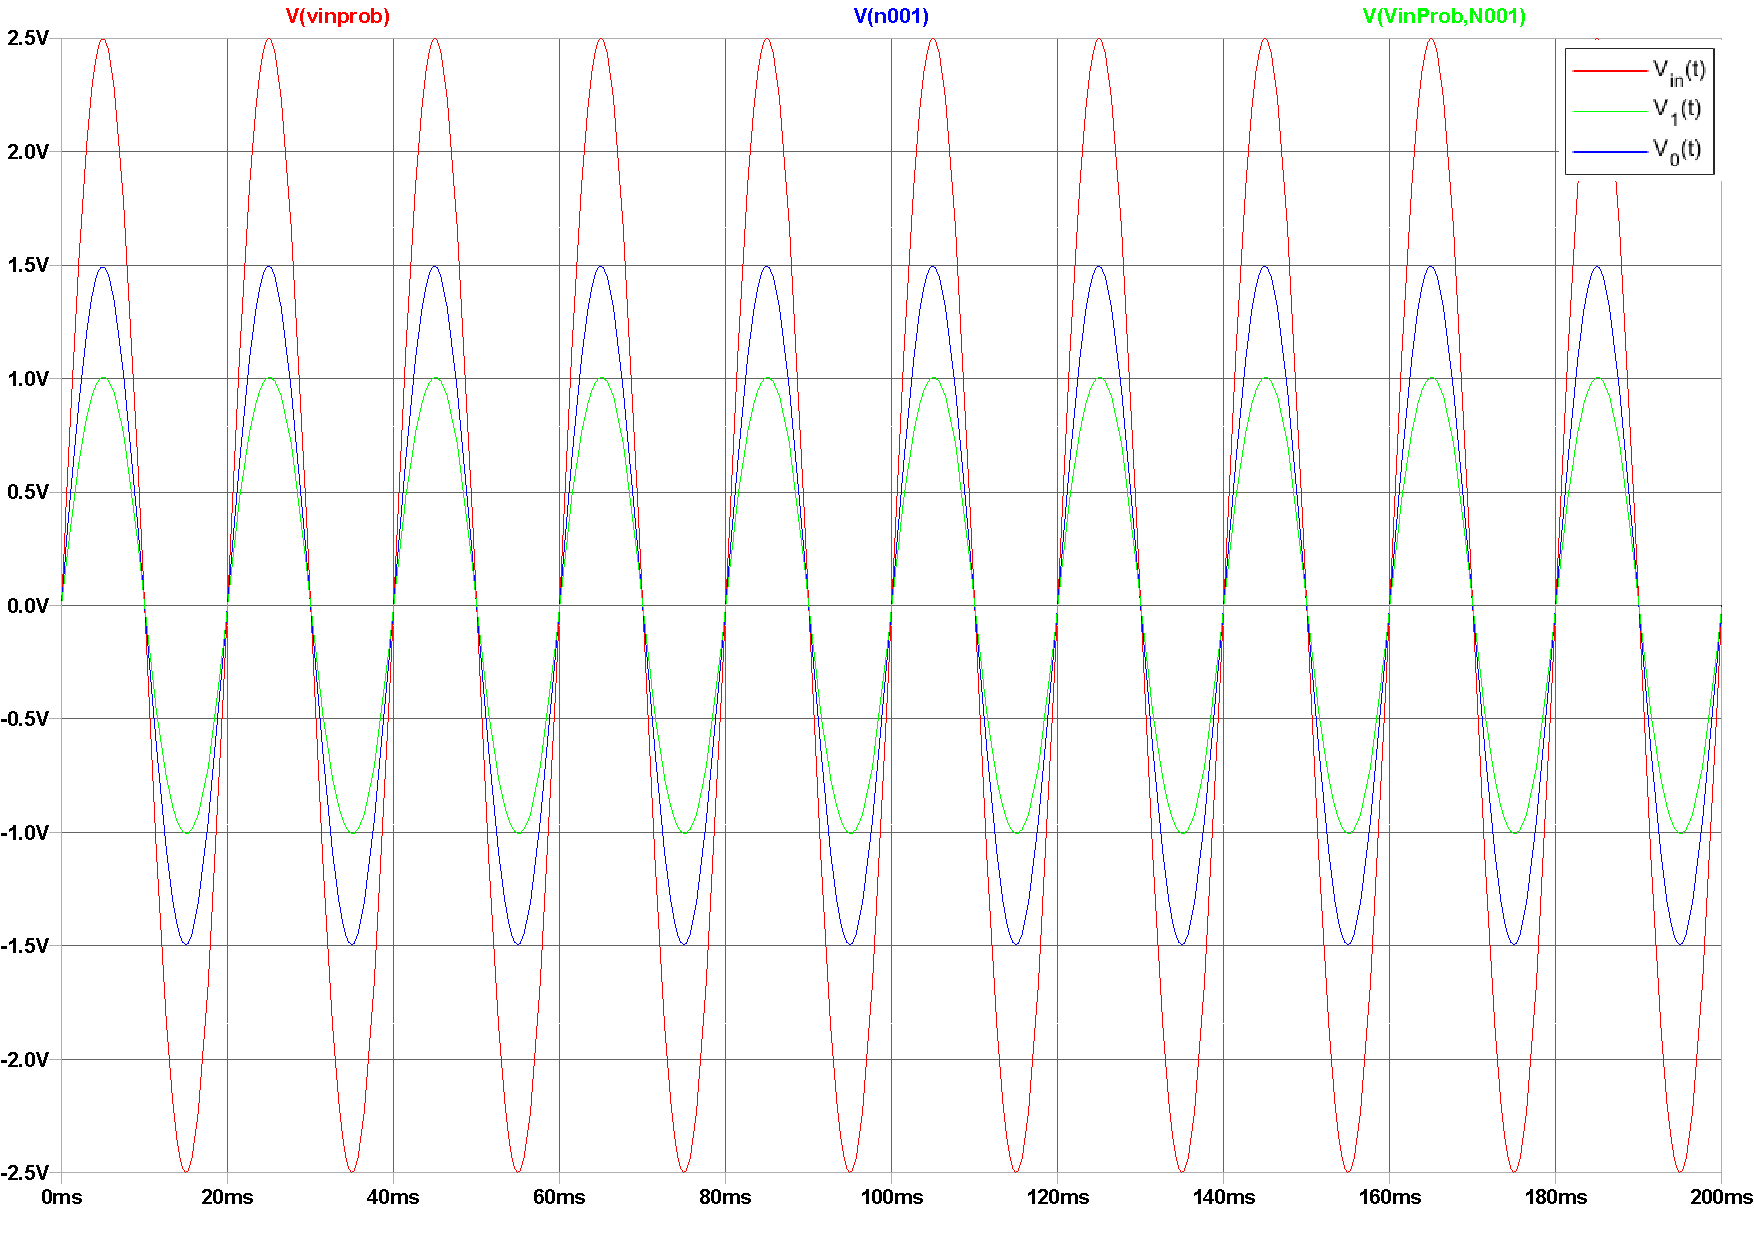
\includegraphics[scale=0.25]{2a_plot.pdf}}
		\caption{Experiment 2}
\end{figure}
	
https://components101.com/sites/default/files/component_datasheet/LDR\%20Datasheet.pdf \\

https://imagine.gsfc.nasa.gov/features/yba/M31_velocity/lightcurve/more.html \\

https://www.analog.com/en/applications/technology/3d-time-of-flight.html \\

https://www.ti.com/lit/an/sbau305b/sbau305b.pdf \\